\documentclass[a4paper,10pt]{report}

\usepackage{url}
\usepackage{graphicx}
\usepackage{verbatim}
\usepackage[usenames,dvipsnames]{color}
\usepackage{listings}
\usepackage{pifont}
\usepackage{bibentry}
\usepackage[margin=12pt,font=small,labelfont=bf]{caption}

% This looks better than CM
\usepackage{palatino}
\usepackage[margin=1.5in]{geometry}

% Colors
\definecolor{Blue}{rgb}{0,0,1}
\definecolor{Red}{rgb}{1,0,0}

% Parameters
\widowpenalty=9999
\clubpenalty=9999

% frequent acronyms, abbreviations, aliases, etc.
\newcommand{\ascii}{\textsc{ascii}}
\newcommand{\cmake}{\textsc{cm}ake}
\newcommand{\css}{\textsc{css}}
\newcommand{\eg}{\textit{e.g.}}
\newcommand{\etc}{etc.}
\newcommand{\gc}{\textsc{gc}}
\newcommand{\gnu}{\textsc{gnu}}
\newcommand{\ie}{\textit{i.e.}}
\newcommand{\lca}{\textsc{lca}}
\newcommand{\libxml}{libxml}
\newcommand{\no}{Newick order}
\newcommand{\nutils}{Newick Utilities}
\newcommand{\nw}{Newick}
\newcommand{\pdf}{\textsc{pdf}}
\newcommand{\phylip}{\textsc{phylip}}
\newcommand{\stderr}{standard error}
\newcommand{\stdin}{standard input}
\newcommand{\stdout}{standard output}
\newcommand{\svg}{\textsc{svg}}
\newcommand{\unix}{\textsc{Unix}}
\newcommand{\xml}{\textsc{xml}}

% names of programs
\newcommand{\clade}{\texttt{nw\_clade}}
\newcommand{\condense}{\texttt{nw\_condense}}
\newcommand{\display}{\texttt{nw\_display}}
\newcommand{\distance}{\texttt{nw\_distance}}
\newcommand{\duration}{\texttt{nw\_duration}}
\newcommand{\ed}{\texttt{nw\_ed}}
\newcommand{\gen}{\texttt{nw\_gen}}
\newcommand{\labels}{\texttt{nw\_labels}}
\newcommand{\luaed}{\texttt{nw\_luaed}}
\newcommand{\match}{\texttt{nw\_match}}
\newcommand{\nwindent}{\texttt{nw\_indent}} % \indent already exists
\newcommand{\order}{\texttt{nw\_order}}
\newcommand{\prune}{\texttt{nw\_prune}} 
\newcommand{\reroot}{\texttt{nw\_reroot}}
\newcommand{\rename}{\texttt{nw\_rename}}
\newcommand{\support}{\texttt{nw\_support}}
\newcommand{\sched}{\texttt{nw\_sched}}
\newcommand{\stats}{\texttt{nw\_stats}}
\newcommand{\topology}{\texttt{nw\_topology}}
\newcommand{\trim}{\texttt{nw\_trim}}

% Arbitrary-size horizontal rules - good for titles
\newcommand{\Hrule}[1]{\rule{\linewidth}{#1}}

\includeonly{simple_tasks}

%\usepackage{hyperref} % shuould come *last*

\begin{document}
\nobibliography*

\begin{titlepage}
\begin{center}
\Hrule{0.5mm} \\[0.8cm]
{\Huge Newick Utilities Tutorial} \\[0.5cm]
Version 1.6.0 -- \today \\
\medskip
Thomas Junier \texttt{thomas.junier@unine.ch} \\
Swiss Institute of Bioinformatics \\
and \\
University of Neuch\^{a}tel, Switzerland \\
\ding{91} \ding{91} \ding{91} \\
but developed (2006-2011) at: \\
Computational Evolutionary Genomics Group \\
Department of Genetic Medicine and Development \\
University of Geneva, Switzerland \\
\medskip
\url{http://cegg.unige.ch/newick_utils}
\Hrule{0.5mm}
\\[2cm]
\includegraphics[width=0.8\textwidth]{title_svg.pdf}
\end{center}
\end{titlepage}

\tableofcontents


\chapter{Introduction}

The \nutils{} are a set of \unix{} shell programs for working with Newick-formatted phylogenetic trees. Their main features are:
\begin{itemize}
 \item they require no user interaction.\footnote{Why this is a good thing is not the focus of this document: I shall assume that if you are reading this, you already know when a command-line interface is better than an interactive interface.}
 \item they can work on any number of trees at a time\footnote{Strictly speaking, a few applications are limited to one input tree because working on more than one is not practical}
 \item they perform reasonably well with large trees
 \item they are implemented as filters
\end{itemize}
They are not tools for \emph{making} phylogenies. Rather, they are for working with existing ones, by which I mean manipulating the tree or extracting information from it: rerooting, simplifying, extracting subtrees, printing branch lengths and distances, etc - a glance at the table of contents of this document should give you an idea.

Each of the programs performs one task (with some variants). For example, here is how you would reroot a series of phylograms contained in file \texttt{mytrees.nw} using node \texttt{Dmelano} as outgroup:

\begin{verbatim}
$ nw_reroot mytrees.nw Dmelano
\end{verbatim} 
Now, you might want to make cladograms from the rerooted trees. Program \topology{} does the job, and since the utilities are filters, you can do it in a single command:
\begin{verbatim}
$ nw_reroot mytrees.nw Dmelano | nw_topology -
\end{verbatim}
As you can see, it is straightforward to pipe \nutils{} together, and of course they can be mixed freely with any other shell tool (see e.g. \ref{sct_counting_leaves}).

This document is organized as follows: chapter \ref{chap_general} discusses common features of the \nutils, chapter \ref{chap_simple} shows examples of simple tasks, and chapter \ref{chap_adv} has examples of more advanced tasks. 




\chapter{General Remarks}
\label{chap_general}

The following applies to all programs in the \nutils{} package.

\section{Help}
\label{sect_help}

All programs print a help message if passed option \texttt{-h}:

\begin{samepage}
\begin{verbatim}
$ nw_indent -h
Indents the Newick, making structure more clear.

Synopsis
--------

nw_indent [-cht:] <newick trees filename|->

Input
-----

Argument is the name of a file that contains Newick trees, or '-' (in
which case trees are read from standard input).

Output
------

By default, prints the input tree, with each parenthesis and each leaf on a
line of its own, and indented a multiple of '  ' (two spaces) to reflect
structure. The default output is valid Newick.
[...]
\end{verbatim}
\end{samepage}
The help page describes the program's purpose, its input and output, and its options, in a format reminiscent of \unix{} manpages. It also shows a few examples. All examples can be tried out using files in the \texttt{data} directory.

\section{Input}
\label{sect_input}

Since the \nutils{} are for working with trees, it should not be a surprise that all programs take Newick as input. The Newick format is a file format for (phylogenetic) trees. It is one of the most widely used and uderstood formats.
A complete description can be found at \url{http://evolution.genetics.washington.edu/phylip/newicktree.html}.

The input tree(s) are always the first argument to the program (after any options). They may either be stored in a file, or piped on \stdin{}. In the latter case, the filename is replaced by a '\texttt{-}' (dash):

\begin{samepage}
\begin{verbatim}
$ nw_display mytrees.nw
\end{verbatim}
is the same as
\begin{verbatim}
$ cat mytrees.nw | nw_display -
\end{verbatim}
\end{samepage}
Of course the second form is only really useful when chaining several programs into pipelines.

\subsection{Multiple Trees in Input}

Most programs can work on any number of trees. That is, in the example above the file \texttt{mytrees.nw} may contain one or more trees, preferably one tree per line\footnote{It may also work if the trees are formatted differently, but the programs were only tested on input files with one tree per line.}. The task will be performed on each tree in the input. So if you need to reroot 1,000 trees on the same outgroup, you can do it all in a single step (see \ref{sct_reroot}).

\section{Output}
\label{sect_output}

The \nutils{} either modify trees and print the result, or print information about the trees. In the first case, the output is also Newick.




\chapter{Simple Tasks}
\label{chap_simple}

The tasks shown in this chapter all involve a single \nutils{} program (plus
possibly \display), so they can serve as introduction to each individual
program.


\section{Displaying Trees}
\label{sct_display}

Perhaps the simplest and most common operation on a \nw{} tree is just to look at it. The \nw{} format is not very easy to understand for us humans, so we have to produce a graphical representation from it. This is the purpose of the \display{} program. 

\subsection{As Text}
\label{sct_display_text}

At the simplest, \display{} just outputs a text graph:
\verbatiminput{dspl1_txt.cmd}
\begin{samepage}
\verbatiminput{dspl1_txt.out}
\end{samepage}
That's pretty low-tech compared to interactive, colorful graphical displays,
but if you use the shell a lot (like I do), you may find it useful.

You can use option \texttt{-w} (``width'') to set the number of columns available for display:

\verbatiminput{dspl2_txt.cmd}
\begin{samepage}
\verbatiminput{dspl2_txt.out}
\end{samepage}

\subsection{As Scalable Vector Graphics (SVG)}
\label{sct_display_svg}

First, a disclaimer: there are dozens of tools for viewing trees out there, and I'm not interested in competing with them. The reason why I added \svg{} capabilities were:
\begin{itemize}
 \item I wanted to be able to produce reasonable graphics even if no other tool was at hand
 \item I wanted to be sure that large trees could be rendered\footnote{I have had serious problems visualising trees of more than 1,000 leaves using some popular software I will not name here - either it was painfully slow, or it simply crashed} 
\end{itemize}
The \svg{} produced by \display{} is designed to be easy to edit in an
interactive editor like Inkscape: the tree edges are in one group, and the text
in another. So it is easy to change the line properties of the edges, or the
font family of the text, for example (you can also do this from \display{}
using a \css{} map, see \ref{sct_display_svg_css}).

To produce \svg, pass option \texttt{-s}:
\begin{verbatim}
$ nw_display -s catarrhini > catarrhini.svg
\end{verbatim}

Now you can visualize the result using any \svg-enabled tool (all good Web browsers can do it), or convert it to another format with, say \texttt{rsvg} or Inkscape. The following image was produced like this:

\begin{verbatim}
$ inkscape -f catarrhini.svg -A catarrhini.pdf
\end{verbatim}

\begin{center}
 \includegraphics{dspl_svg1_svg.pdf}
\end{center}

All \svg{} images shown in this document were produced in the same way, although from now on we will generally omit the \svg{} to \textsc{pdf} conversion step.

There are many options for \svg{} graphs.First, you can make radial trees, using option \texttt{-r} (from now on I will skip the redirection into an \svg{} file):

\verbatiminput{dspl_sr_w450_catarrhini_svg.cmd}

You already know \texttt{-w}, except that for \svg{} the value is in pixels instead of columns. 

\begin{center}
\includegraphics{dspl_sr_w450_catarrhini_svg.pdf}
\end{center}

\subsubsection{Using \css}
\label{sct_display_svg_css}

You can modify node style using \css. This is done by specifying a
\textit{\css{} map}, which is just a text file that says which style should be
applied to which node. If file \texttt{css.map} contains the following
\begin{quote} \verbatiminput{css.map} \end{quote} we can apply the style map to
the tree above:

\verbatiminput{nw_display_sr_w450_ccssmap_catarrhini_svg.cmd}

\begin{center}
 \includegraphics{nw_display_sr_w450_ccssmap_catarrhini_svg.pdf}
\end{center}

The syntax of the \css{} map is as follows. Each line describes one style and the set of nodes to which it applies. The first line in \texttt{css.map} says that the style \texttt{stroke-width:2;stroke:blue} must be applied to the \texttt{Clade} defined by \texttt{Homo} and \texttt{Pan}, which comprises \texttt{Homo}, \texttt{Pan}, and \texttt{Hominini}. The \texttt{Clade} keyword can be abbreviated to \texttt{C}, as in the next two lines. The style of an inner clade overrides styles of an outer clade, \textit{e.g.}, although the \texttt{Homo} - \texttt{Pan} clade is nested inside the \texttt{Homo} - \texttt{Hylobates} clade, it has its own style (blue, wide lines) which overrides the containing clade's style (pinkish with normal width).

The \texttt{Individual} keyword specifies that the style is to be applied to all nodes who match the labels on the line, but individually, that is, the program does not propagate the style to the whole clade defined by the labels. This is why only \texttt{Colobus} and \texttt{Cercopithecus} appear in green; with the \texttt{Clade} keyword the whole \texttt{Macaca} - \texttt{Colobus} clade (that is, all Old-World monkeys) would be green. Note that \texttt{Individual} overrides \texttt{Clade}, which is why \texttt{Cercopithecus} is green even though it belongs to a red clade.

The \texttt{Clade} and \texttt{Individual} keywords are not case-sensitive and can be abbreviated - in fact only the first letter counts.

Styles can also be applied to labels. Option \texttt{-l} specifies the leaf
label style, option \texttt{-i} the inner node label style, and option
\texttt{-b} the branch length style. For example, the following tree, which was
produced using defaults, could be improved a bit:

\verbatiminput{nw_display_s_vertebrata_svg.cmd}
\begin{center}
  \includegraphics{nw_display_s_vertebrata_svg.pdf}
\end{center}

\noindent{}Let's remove the branch length labels, reduce
the vertical spacing, reduce the size of inner node labels (bootstrap values),
and write the leaf labels in italics, using a font with serifs:
\verbatiminput{nw_display_s_vertebrata_styled_svg.cmd}
\begin{center}
  \includegraphics{nw_display_s_vertebrata_styled_svg.pdf}
\end{center}
Option \texttt{-v} specifies the vertical spacing, in pixels, between two
successive leaves (the default is 40). Option \texttt{-b} sets the style of
branch labels, option \texttt{-l} sets the style of leaf labels, and option
\texttt{-i} sets the style of inner node labels. Note that we did not
\emph{discard} the branch lengths (we could do this with \topology), because
doing so would reduce the tree to a cladogram. Instead, we set their \css{}
style to \texttt{opacity:0} (\texttt{visibility:hidden} also works).

\subsection{Ornaments}

Ornaments are arbitrary snippets of \svg{} code that are displayed at specified
node positions. As for \css, this is done with a map. The ornament map has the
same syntax as the \css{} map, except that you specify \svg{} objects rather
than \css{} styles. In particular, the \texttt{Individual} and \texttt{Clade}
keywords have the same meaning, and can be abbreviated in the same way. The
following file, \texttt{ornament.map}, instructs to draw a red circle with a
black border on \texttt{Homo} and \texttt{Pan}, and a cyan circle with a blue
border on the root of the \texttt{Homo} - \texttt{Hylobates} clade. The \svg{} is enclosed in double quotes because it contains spaces. The
ornament map is specified with option \texttt{-o}:
				
\begin{quote}
 \verbatiminput{ornament.map}
\end{quote}

\verbatiminput{nw_display_sr_w450_oornmap_catarrhini_svg.cmd}

\begin{center}
 \includegraphics{nw_display_sr_w450_oornmap_catarrhini_svg.pdf}
\end{center}

\noindent{}The \css{} map and ornaments can be combined:

\verbatiminput{nw_display_sr_w450_oornmap_ccssmap_catarrhini_svg.cmd}

\begin{center}
 \includegraphics{nw_display_sr_w450_oornmap_ccssmap_catarrhini_svg.pdf}
\end{center}

\subsubsection{Multiple \svg{} Trees}

Like all \nutils, \display{} can handle multiple trees, even in \svg{} mode.
The best way to do this is not evident: one can generate one file per tree (but
then we break the rule that every program is a filter and so writes to standard
output), or one can put all the trees in one \svg{} document (but then we have
to impose tiling or some other arrangement), or one can just output one \svg{}
document after another. This is what we do (this may change in the future). So
if you have many trees in document \texttt{forest.nw}, you can say:
\begin{quote}
\verb+$ nw_display -s forest.nw > forest_svg+
\end{quote}
But \texttt{forest\_svg} isn't valid \svg{} -- it is a concatenation of many \svg{} documents. You can just extract them into individual files with \texttt{csplit}:
\begin{quote}
\verb+$ csplit -sz -f tree_ -b '%02d.svg' forest_svg '/<?xml/' {*}+
\end{quote}
This will produce one \svg{} file per tree in \texttt{forest.nw}, named \texttt{tree\_01.svg}, \texttt{tree\_02.svg}, etc.

\subsection{Options not Covered}

\display{} has many options, and we will not describe them all here - all of
them are described when you pass option \texttt{-h}. They include support for
clickable images (with URLs to arbitrary Web pages), setting the scale bar
units, changing the root length, etc. 



\section{Rooting and Rerooting}
\label{sct_reroot}

Rooting transforms an unrooted tree into a rooted one, and rerooting changes a rooted tree's root. Some tree-building methods produce rooted trees (e.g., \textsc{upgma}), others produce unrooted ones (neighbor-joining, maximum-likelihood). 

The Newick format is implicitly rooted, in the sense that there is a 'top' node from which all other nodes descend. Some applications regard a tree with a trifuraction at the top node as unrooted. 

Rooting a tree is usually done by specifying an \textit{outgroup}. In the simplest case, this is a single leaf. The root is then placed in such a way that one of its children is the outgroup, while the other child is the rest of the tree (sometimes known as the \textit{ingroup}). 

Consider the following primate tree, \texttt{simiiformes\_wrong}:

\includegraphics{reroot_1_svg.pdf}

\noindent{}It is wrong because \texttt{Cebus}, which is a New World monkey (capuchin), should be the sister group of all the rest (Old World monkeys and apes, technically Catarrhini), whereas it is shown as the sister group of the macaque-colobus family, Cercopithecidae. We can correct this by re-rooting the tree using \texttt{Cebus} as outgroup:
\verbatiminput{reroot_2_svg.cmd}
which produces:

\includegraphics{reroot_2_svg.pdf} \\

\noindent{}Note that the root is placed in the middle of the ingroup-outgroup
edge.

The outgroup does not need to be a single leaf. The following tree is
wrong for the same reason as the one before, except that is has three New World
monkey species instead of one, and they appear as a clade (Platyrrhini) in the
wrong place:

\includegraphics{reroot_3_svg.pdf} \\

\noindent{}We can correct this by specifying the New World monkey clade as outgroup:

\verbatiminput{reroot_4_svg.cmd}

\includegraphics{reroot_4_svg.pdf} \\

\noindent{}Note that I did not include all three New World monkeys, only \texttt{Cebus} and \texttt{Allouatta}. This is because it is always possible to define a clade using only two leaves. The result would be the same if I had included all three, though. You can use inner labels too, if there are any:
\begin{verbatim}
$ nw_reroot simiiformes_wrong_3og Platyrrhini
\end{verbatim}
will reroot in the same way (not shown). Beware that inner labels are often
used for support values (as in bootstrapping), which are generally not useful
for defining clades.

\subsection{Rerooting on the ingroup}

Sometimes the desired species cannot be used for rooting, as their last common ancestor is the tree's root. For example, consider the following tree:

\includegraphics{reroot_5_svg.pdf}

\noindent{}It is wrong because \textit{Danio} (a ray-finned fish) is shown
closer to tetrapods than to other ray-finnned fishes (\textit{Fugu} and
\textit{Tetraodon}). So we should reroot it, specifying that the fishes should
form the outgroup. We could try this:

\verbatiminput{reroot_6_txt.cmd}

\noindent{}But this will fail:

\verbatiminput{reroot_6_txt.out}

\noindent{}This fails because the last common ancestor of the two pufferfish is
the root itself. The workaround in this case is to try the ingroup. This is
done by passing option \texttt{-l} ("lax"), along with \emph{all} species in the
outgroup (this is because \reroot{} finds the ingroup by complementing the outgroup):

\verbatiminput{reroot_7_svg.cmd}
\includegraphics{reroot_7_svg.pdf}

\noindent{}To repeat: all outgroup labels were passed, not just the two
normally needed to find the last common ancestor -- since, precisely, we can't
use the \lca.




\section{Extracting Subtrees}
\label{sct_subtrees}

You can extract a clade from a tree with \clade. A clade is specified by a
number of labeled, as usual (see \ref{sct_def_clades}).

We'll use the catarrhinian tree again for these examples, so here it is.

\begin{center}
\includegraphics{dspl_sr_w450_catarrhini_svg.pdf}
\end{center}

 In the simplest case, the clade you want to extract has its own, unique label.
This is the case of \texttt{Cercopithecidae}, so you can extract the whole
cercopithecids (Old World monkeys) using just that label:

\verbatiminput{clade1_svg.cmd}
\begin{center}
  \includegraphics{clade1_svg.svg}
\end{center}


\section{Computing Bootstrap Support}

\support{} computes bootstrap support values from a target tree and a file of
replicate trees. Say the target tree is in file \texttt{HRV.nw} and the
replicates (20 of them) are in \texttt{HRV\_20reps.nw}. You can attribute
support values to the target tree like this:

\verbatiminput{support_1_svg.cmd}
\includegraphics{support_1_svg.pdf}

\noindent{}In this case I have colored the support values red. Option
\texttt{-p} uses percentages instead of absolute counts.

\subsubsection{Notes}

There are many tree-building programs that compute bootstrap support. For
example, PhyML can do it, but for large tasks I typically have to distribute
the replicates over several jobs (say, 100 jobs of 10 replicates each). I then
collect all replicates files, concatenate them, and use \support{} to attribute
the values to the target tree.

\support{} assumes rooted trees (it may as well, since \nw{} is implicitly
rooted), and the target tree and replicates should be rooted the same way. Use
\reroot{} to ensure this.


\section{Retaining Topology}
\label{sct_topology}

There are cases when one is more interested in the tree's structure than in the
branch lengths, maybe because lengths are irrelevant or just because they are
so short that they obscure the branching order. Consider the following tree:
\begin{samepage}
\verbatiminput{topol_1_txt.out}
\end{samepage}
Its structure is not evident, particularly in the upper half. This is because
many branches are short in relation to the depth of the tree, so they are not
well resolved. A better-resolved tree can be obtained by discarding branch
lengths altogether:
\verbatiminput{topol_2_txt.cmd}
\begin{samepage}
\verbatiminput{topol_2_txt.out}
\end{samepage}
This effectively produces a \emph{cladogram}, that is, a tree that represents
ancestry relationships but not rates of evolutionary change. The inner nodes are
evenly spaced over the depth of the tree, and the leaves are aligned, so the
branching order is more apparent.

Of course, \ascii{} trees have low resolution in the first place, so I'll show
both trees look in \svg. First the original: 
\verbatiminput{topol_3_svg.cmd}
\includegraphics{topol_3_svg.pdf} \\

\noindent{}And now as a cladogram:
\verbatiminput{topol_4_svg.cmd}
\includegraphics{topol_4_svg.pdf} \\
As you can see, even with \svg{}'s much better resolution, it can be useful to
display a tree as a cladogram.

\topology{} has the following options: \texttt{-b} keeps the branch lengths (obvioulsy, using this option alone has no effect); \texttt{-I} discards inner node labels, and \texttt{-L} discards leaf labels. An extreme example is the following, which discards everything \emph{but} topology:
\verbatiminput{topol_5_txt.cmd}
This produces the following tree, which is still valid Newick:
\verbatiminput{topol_5_txt.out}
Let's look at it as a radial tree, for a change:
\verbatiminput{topol_6_svg.cmd}
\includegraphics{topol_6_svg.pdf}



\section{Extracting Distances}

There are many ways of defining distances in a tree. First, we have to consider
whether the tree is a cladogram or a phylogram: in the former case, the
distances will be measured in whatever units the tree was built with (usually
substitutions per site), in the latter, it will just be the number of ancestors.

Then we can measure distance in a variety of ways. This is the job of
\distance. By default, it prints the distance from the root of the tree to all
labeled leaves, in the order in which they appear in the Newick. Let's look at
distances in the monkeys tree:

\begin{center}
\includegraphics{dspl_svg1_svg.pdf}
\end{center}

\verbatiminput{dist_1_txt.cmd}
\begin{samepage}
\verbatiminput{dist_1_txt.out}
\end{samepage}
This means that the distance from the root to \texttt{Gorilla} is 56, etc. Option \texttt{-n} shows the labels:
\verbatiminput{dist_2_txt.cmd}
\begin{samepage}
\verbatiminput{dist_2_txt.out}
\end{samepage}

There are two main parameters to \distance: the \emph{method} and the
\emph{selection}. The method determines how to compute the distance (from what
node to what node), and the selection determines for which nodes the program is
to compute distances. Let's look at examples.

\subsection{Selection}

In this section we will show the different selections, using the default
distance method. The selection type is the argument to option \texttt{-s}.
The nodes appear in the same order as in the Newick tree, except when they are
specified on the command line (see below).

To illustrate the selection types, we need a tree that has both labeled and
unlabeled leaves and inner nodes. Here it is in Newick format (I indented it
with \nwindent{} - see \ref{sct_indent}):
\verbatiminput{dist_sel_xpl.nw}
And here it is in graphical form:
\begin{center}
\includegraphics{dist_3_svg.pdf}
\end{center}
We will use option \texttt{-n} to see the node labels.

\subsubsection{All labeled leaves}

The selection consists of all leaves with a label. This is the default, as
leaves will mostly be labeled and we're generally more interested in leaves
than inner nodes.
\verbatiminput{dist_4_txt.cmd}
\verbatiminput{dist_4_txt.out}

\subsubsection{All labeled nodes}

Option \texttt{-s l}. This takes all labeled nodes into account, whether they are leaves or inner nodes.
\verbatiminput{dist_5_txt.cmd}
\verbatiminput{dist_5_txt.out}

\subsubsection{All leaves}

Option \texttt{-s f}. Selects all leaves, whether they are
labeled or not.
\verbatiminput{dist_6_txt.cmd}
\verbatiminput{dist_6_txt.out}

\subsubsection{All nodes}

Option \texttt{-s a}. All nodes are selected.
\verbatiminput{dist_7_txt.cmd}
\verbatiminput{dist_7_txt.out}

\subsubsection{Command line selection}

The selection consists of the nodes whose labels are passed as arguments on
the command line (after the file name). 
\verbatiminput{dist_8_txt.cmd}
\verbatiminput{dist_8_txt.out}

\subsection{Methods}

In this section we will take the default selection and vary the method. The
method is te argument to option \texttt{-m}.

\subsubsection{Distance from the Tree's Root}

This is the default method: for each node in the selection, the program prints
the distance from the tree's root to the node. This was shown above, so I
won't repeat it here.

\subsubsection{Distance from last common ancestor}






\section{Renaming nodes}
\label{sct_rename}

Renaming nodes is the rather boring operation of changing a node's label. It
can be done \eg{} for the following reasons:
\begin{itemize}
	\item building a higher-level tree (\ie, a families tree from a tree of genera, etc)
	\item mapping one namespace into another (see \ref{sct_10_char_limit})
	\item correcting wrong names
\end{itemize}

\noindent{}Renaming is done with \rename. This takes a \emph{renaming map},
which is just a text file with the old and new names on the same line.

\subsection{Breaking the 10-character limit in \phylip{} alignments}
\label{sct_10_char_limit}

A technical hurdle with phylogenies is that some programs do not accept names
longer than, say, 10 characters in the \phylip{} alignment. But of
course, many scientific names or sequence \textsc{ID}s are longer than that.
One solution is to rename the sequences, before constructing the tree, using a
numerical scheme, \eg{}, \textit{Strongylocentrotus purpuratus} $\rightarrow$
\texttt{ID\_01}, etc. This means we have an alignment of the following form:
\begin{verbatim}
 154 259
ID_01     PTTSNSAPAL DAAETGHTSG ...
ID_02     SVSSHSVPAL DAAETGHTSS ...
...
\end{verbatim}
together with a renaming map, \texttt{id2longname.map}:
\begin{verbatim}
ID_01	Strongylocentrotus_purpuratus
ID_02	Harpagofututor_volsellorhinus
...
\end{verbatim}
The alignment's \textsc{ID}s are now sufficiently short, and we can use it to
make a tree. It will look something like this:

\verbatiminput{rename_1_svg.cmd}
\begin{center}
\includegraphics{rename_1_svg.pdf}
\end{center}

\noindent{}Not very informative, huh? But we can put back the original, long
names (option \texttt{-W} specifies the mean width of label characters, in
pixels -- use it when the default is wrong, as in this case with very long
labels and small characters):

\verbatiminput{rename_2_svg.cmd}
\begin{center}
\includegraphics{rename_2_svg.pdf}
\end{center}

\noindent{}Now that's better\ldots although exactly what these critters are
might not be evident. Not to worry, I've made another map and I can rename the
tree a second time on the fly:

\verbatiminput{rename_3_svg.cmd}
\begin{center}
\includegraphics{rename_3_svg.pdf}
\end{center}

\subsection{Higher-rank trees}
\label{sct_higher_rank}

Here is a tree of a few dozen enterovirus and rhinovirus isolates. I show it as
a cladogram (using \topology, see \ref{sct_topology}) because branch lengths do
not matter here. I know that these isolates belong to three species in two
genera: human rhinovirus A (\texttt{hrv-a}), human rhinovirus B
(\texttt{hrv-b}, and enterovirus (\texttt{hev}). 

\verbatiminput{rename_4_svg.cmd}
\begin{center}
\includegraphics{rename_4_svg.pdf}
\end{center}

\noindent{}I want to see if the tree correctly groups isolates of the same
species together. So I use a renaming map that maps an isolate name to its
species:
\begin{verbatim}
HRV16 HRV-A
HRV1B HRV-A
...
HRV37 HRV-B
HRV14 HRV-B
...
POLIO1A HEV
COXA17 HEV
\end{verbatim}

\verbatiminput{rename_5_svg.cmd}
\begin{center}
\includegraphics{rename_5_svg.pdf}
\end{center}

\noindent{}As we can see, they do. This would be even better if we could
somehow simplify the tree so that clades of the same species were reduced to a
single leaf. And, that's exactly what \condense{} does (see below).


\section{Condensing}
\label{sct_condense}

Condensing a tree means reducing its size in a systematic, meaningful way
(compare this to \emph{pruning} (\ref{sct_prune}) which arbitrarily removes
branches, and to \textit{trimming} (\ref{sct_trim}) which cuts a tree at a
specified depth). Currently the only condensing method available is
simplifying clades in which all leaves have the same label - for example
because they belong to the same taxon, etc. Consider this tree:

[TODO: use HRV tree from section above]

\begin{center}
\includegraphics{condense_1_svg.pdf}
\end{center}

\noindent{}it has a clade that consists only of A, another of only C, plus a B
leaf.  Condensation will replace those clades by an A and a C leaf,
respectively:

\verbatiminput{condense_2_svg.cmd}
\begin{center}
\includegraphics{condense_2_svg.pdf}
\end{center}

\noindent{}Now the A and B leaves stand for whole clades. The tree is simpler,
but the information about th erelationships of A, B and C is conserved, while
the details of the A and C clades is not.  A typical use of this is producing
genus trees from species trees (or any higher-level tree from a lower-level
one), or checking consistency with other data -- see \ref{sct_higher_lvl}).

Condensing the virus tree of section \ref{sct_rename_species} gives this:

\includegraphics{condense_3_svg.pdf}

\noindent{}The relationships between the species is now evident -- as is the
fact that the various isolates do cluster within species in the first place.
This need not be the case, and renaming-then-condensing is a useful technique
for checking this kind of consistency in a tree (see
\ref{sct_check_consistency}) for more examples.


\section{Pruning}
\label{sct_prune}

Pruning is simply removing arbitrary nodes. Say you have the following tree (as
it happens, it contains a glaring error since the sister clade of mammals is the
amphibian rather than the bird):

\begin{center}
\includegraphics{prune_1_svg.pdf}
\end{center}

\noindent{}and say you only need a subset of the species, perhaps because you
want to compare this tree to another tree with fewer species. Specifically,
let's say you don't need to show \textit{Tetraodon}, \textit{Danio},
\textit{Bombina}, and \textit{Didelphis}. You just pass those labels to
\prune:

\verbatiminput{prune_2_svg.cmd}
\begin{center}
\includegraphics{prune_2_svg.pdf}
\end{center}

\noindent{}Note that each label is removed individually. The discarding of
\textit{Didelphis} is the cause of the disappearance of the node labeled
Mammalia. And the embarrassing error is hidden by the removal of
\textit{Bombina}.

You can also discard internal nodes, if they are labeled (in future versions
it will be possible to discard a clade by specifying descendants, just like
\clade). For example, you can discard the whole mammalian clade like this:

\verbatiminput{prune_3_svg.cmd}
\begin{center}
\includegraphics{prune_3_svg.pdf} 
\end{center}

By the way, \textit{Tetrao} and \textit{Tetraodon} are not the same thing, the
first is a bird (grouse), the second is a pufferfish.

\subsection{Keeping selected Nodes}

By passing option \texttt{-v} (think of \texttt{grep -v}), the nodes whose
labels are passed are \emph{kept}, and the other ones are discarded (except
unlabeled nodes). And I really mean this: if a node's label is not on the
command line, it goes away, even if it is an inner node - this can have
surprising results.\footnote{In future versions there will be an option for
finer control of this behaviour}.

Suppose I think that the tree is unfairly biased towards mammals (and in a
lesser way, actinopterygians), and want to keep only the following genera:
\textit{Fugu}, \textit{Tetrao}, \texttt{Bombina}, \textit{Sorex}. I could, of
course, generate the list of all leaves that must go away, but it is easier to
do this:

\verbatiminput{prune_4_svg.cmd}
\begin{center}
\includegraphics{prune_4_svg.pdf} 
\end{center}

\noindent{}Note that I also passed \texttt{Mammalia}, for the reason discussed
above: the node with this label would go away if I did not, resulting in a
different tree (try it out).



\section{Indenting}
\label{sct_indent}

\nwindent{} reformats \nw{} on several lines, with one node per line,
nodes of the same depth in the same column, and children nodes to the right of
their parent. This shows the structure more
clearly than the compact form, but since whitespace is ignored in the Newick
format\footnote{except between quotes}, the
indented form is still valid. For example, this is a tree in compact form, in
file \texttt{falconiformes}:
\verbatiminput{falconiformes}
And this is the same tree, indented:
\begin{samepage}
\verbatiminput{indent_1_nw.cmd}
\verbatiminput{indent_1_nw.out}
\end{samepage}
The structure is much more clear, it is also relatively easy to edit manually
in a text editor - while still being valid \nw.

Another advantage of indenting is that it is resistant to certain errors
which would cause \display{} to fail.\footnote{This is
because indenting is a purely lexical process, hence it does not need a
syntactically correct tree.} For example, there is an error in this tree:
\verbatiminput{falconiformes_error}
yet it is hard to spot, and trying \display{} won't help as it will abort with a
parse error. With \nwindent{}, however, you can at least look at the tree:
\begin{samepage}
\verbatiminput{indent_4_nw.out}
\end{samepage}
While the error is not exactly obvious, you can at least view the Newick. It turns out there is a comma missing after \texttt{Sagittarius:5}.

The indentation can be varied by supplying a string (option \texttt{-t}) that
will be used instead of the default (which is two spaces). If you want to
indent by four spaces instead of two, you could say this:
\begin{samepage}
\verbatiminput{indent_2_nw.cmd}
\verbatiminput{indent_2_nw.out}
\end{samepage}
Option \texttt{-t} can also be used to highlight indentation:
\begin{samepage}
\verbatiminput{indent_3_txt.cmd}
\verbatiminput{indent_3_txt.out}
\end{samepage}
Now the indentation levels are easier to see, but at the expense of the tree no
longer being valid \nw.

Finally, option \texttt{-c} ("compact") does the reverse: it removes all
indentation and produces a compact tree. You can use this when you want to
produce a compact Newick file after editing. For example, using Vim, after
loading a \nw{} tree I do 
\begin{quote}
\verb+gg!}nw_indent -+
\end{quote}
to indent the file, then I edit it, then compact it again:
\begin{quote}
\verb+gg!}nw_indent -c -+
\end{quote}




\section{Extracting Labels}
\label{sct_labels}

To get a list of all labels in a tree, use \labels:

\verbatiminput{labels_xpl1_txt.cmd}
\verbatiminput{labels_xpl1_txt.out}

\noindent{}The labels are printed out in post-order. To get rid of internal labels, use \texttt{-I}:

\verbatiminput{labels_xpl2_txt.cmd}
\verbatiminput{labels_xpl2_txt.out}

\noindent{}Likewise, you can use \texttt{-L} to get rid of leaf labels (not shown). Finally, if you use \texttt{-t} the labels are printed on a single line, separated by tabs (for some reason the tabs show as spaces here, I think this is an effect of \LaTeX{}'s \verb+\verbatiminput{}+):

\verbatiminput{labels_xpl3_txt.cmd}
\verbatiminput{labels_xpl3_txt.out}

\subsection{Counting Leaves in a Tree}
\label{sct_counting_leaves}

A simple application of \labels{} is a leaf count (assuming each leaf is
labeled - \nw{} does not require labels):

\verbatiminput{labels_xpl4_txt.cmd}
\verbatiminput{labels_xpl4_txt.out}




\chapter{Advanced Tasks}
\label{chap_adv}

The tasks presented in this chapter are more involved than that of chapter
\ref{chap_simple}, and generally involve many \nutils{} as well as other
programs.

\section{Bootscanning}
\label{sct_bootscanning}

Bootscanning is a technique for finding recombination breakpoints in a
sequence. It involves aligning the sequence of interest (called \emph{query} or
\emph{reference}) with related sequences (including the putative recombinant's
parents) and computing phylogenies locally over the alignment. Recombination is
expected to cause changes in topology.  The tasks involved are shown below:
\begin{enumerate}
\item align the sequences $\rightarrow$ multiple alignment
\item slice the multiple alignment $\rightarrow$ slices
\item build a tree for each slice $\rightarrow$ trees
\item extract distance from query to other sequences (each tree) $\rightarrow$ tabular data
\item plot data $\rightarrow$ graphics
\end{enumerate}
The distribution contains a script, \texttt{src/bootscan.sh}, that performs the whole process. Here is an example run:
\begin{verbatim}
$ bootscan.sh HRV_3UTR.dna HRV-93 CL073908
\end{verbatim}
where \texttt{HRV\_3UTR.dna} is a FastA file of (unaligned) sequences, \texttt{HRV-93} is the outgroup, and \texttt{CL073908} is the query.  Here is the result:

\begin{centering}
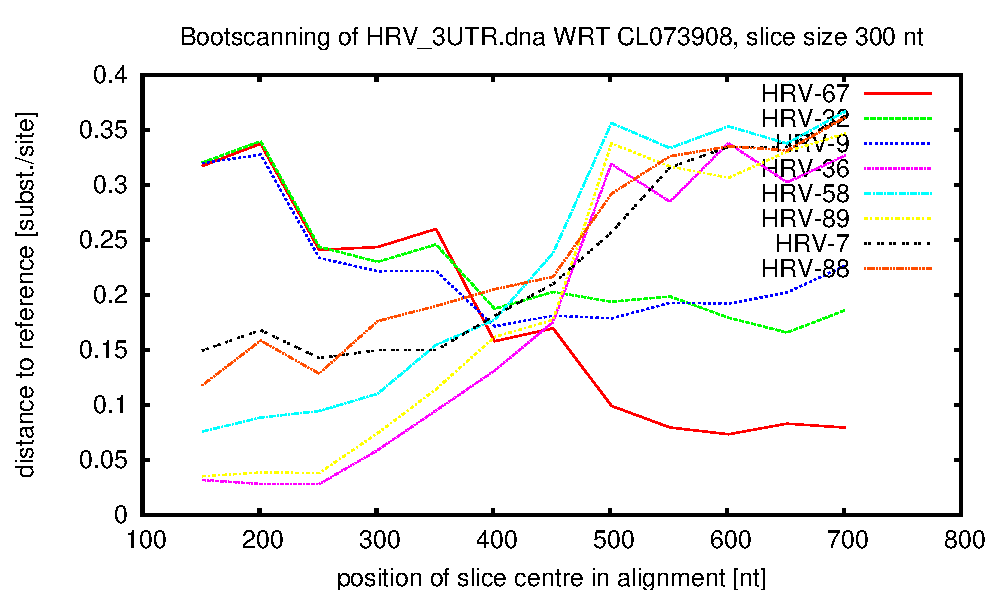
\includegraphics[width=\textwidth]{bootscan_1.pdf}
\end{centering}

\smallskip{}
\noindent{}until position 450 or so, the query sequence's nearest relatives (in
terms of substitutions/site) are \texttt{HRV-36} and \texttt{HRV-89}. After
that point, it is \texttt{HRV-67}. This suggests that there is a recombination
breakpoint near position 450.

The script uses \reroot{} to reroot the trees on the outgroup, \clade{} and
\labels{} to get the labels of the ingroup, \distance{} to extract the distance
between the query and the other sequences, as well as the usual \texttt{sed}, \texttt{grep}, etc. The plot is done with gnuplot.


\section{Number of nodes vs. Tree Depth}
\label{clades_vs_depth}

A simple measure of a tree's shape can be obtained by computing the number of
nodes as a function of depth. Consider the following trees:

\begin{tabular}{ccc}
\includegraphics{clades_vs_depth_1_svg.pdf}
\includegraphics{clades_vs_depth_2_svg.pdf}
\includegraphics{clades_vs_depth_3_svg.pdf}
\end{tabular}


\section{Checking Consistency with other Data}
\label{sct_check_consistency}

\subsection{By condensing}

One can check the consistency of a tree with respect to additional information
by renaming and condensing. For example, I have the following tree of
Falconiformes (diurnal raptors: eagles, falcons, etc):

\includegraphics{higher_lvl_1_svg.pdf}

\noindent{}Now I also have the following information about the family to which each genus belongs:

\bigskip{}
\begin{tabular}{ll}
\textbf{Genus} & \textbf{Family} \\
\textit{Accipiter} & Accipitridae \\
\textit{Aquila} & Accipitridae \\
\textit{Buteo} & Accipitridae \\
\textit{Elanus} & Accipitridae \\
\textit{Falco} & Falconidae \\
\textit{Haliaeetus} & Accipitridae \\
\textit{Micrastur} & Falconidae \\
\textit{Milvago} & Falconidae \\
\textit{Milvus} & Accipitridae \\
\textit{Pandion} & Pandionidae \\
\textit{Polyborus} & Falconidae \\
\textit{Sagittarius} & Sagittariidae
\end{tabular}
\bigskip{}

Let's see if the tree is consistent with this information. If it is, all
families should form clades. To check this, I will rename each leaf by
replacing the genus name by the family name, then condense the tree. If the
original) tree is consistent, the final tree should have one leaf per family.

First, I create a renaming map (see \ref{sct_rename}) based on the above
information (here are the first three lines):
\verbatiminput{higher_lvl_2_txt.cmd}
\verbatiminput{higher_lvl_2_txt.out}
Then I use it to rename, and then I condense the tree:
\verbatiminput{higher_lvl_3_svg.cmd}
\includegraphics{higher_lvl_3_svg.pdf}

\bigskip{}
\noindent{}As we can see, there is one leaf per family, so the above
information is consistent with the tree.

Let's see if common English names are also consistent with the tree. Here is
one possible table of vernacular names of the raptor genera: 

\bigskip{}
\begin{tabular}{ll}
\textbf{Genus} & \textbf{English name} \\
\textit{Accipiter} & hawk (sparrowhawk, goshawk, etc)\\
\textit{Aquila} & eagle  \\
\textit{Buteo} & hawk \\
\textit{Elanus} & kite \\
\textit{Falco} & falcon \\
\textit{Haliaeetus} & eagle (sea eagle) \\
\textit{Micrastur} & falcon (forest falcon)\\
\textit{Milvago} & caracara \\
\textit{Milvus} & kite \\
\textit{Pandion} & osprey \\
\textit{Polyborus} & caracara \\
\textit{Sagittarius} & secretary bird
\end{tabular}
\bigskip{}

And here is the corresponding tree:

\verbatiminput{higher_lvl_4_svg.cmd}
\includegraphics{higher_lvl_4_svg.pdf}
\bigskip{}

So the above common names are consistent with the tree. However, some species
have many common names. For example, the \textit{Buteo} hawks are often called
"buzzards" (in Europe), and two species of falcons have been called "hawks" (in
North America): the peregrine falcon (\textit{Falco peregrinus}) was called the
"duck hawk", and the American kestrel (\textit{Falco sparverius}) was called
the "sparrow hawk".\footnote{This is confusing because there are true hawks
called "sparrow hawks", \emph{e.g.} the Eurasian sparrow hawk \textit{Accipiter
nisus}. To add to the confusion, the specific name \textit{sparverius} looks
like the English word "sparrow", and also resembles the common name of
\textit{Accipiter nisus} in many other languages: \textit{\'{e}pervier} (fr), \textit{Sperber} (de), \textit{sparviere} (it). Oh well. Let's not drop scientific names just yet!} If we
map these common names to the tree and condense, we get this:

\verbatiminput{higher_lvl_5_svg.cmd}
\includegraphics{higher_lvl_5_svg.pdf}
\bigskip{}

\noindent{}Distinguishing buzzards from other hawks fits well with the tree. On
the other hand, calling a falcon a hawk does not, and the name "hawk" appears
in two different places.



\lstset{
	language=Python,
	basicstyle=\ttfamily,
	keywordstyle=\color{NavyBlue},
	stringstyle=\color{OliveGreen},
	commentstyle=\color{red},
	frame=single,
	frameround=tttt,
	framexleftmargin=8mm,
	numbers=left
}

\chapter{Python Bindings}
\label{chap_python_lib}

This chapter shows how you can use the \nutils{}'s functionalities in Python
programs. While the \nutils{} are written in C, the \texttt{ctypes}
module\footnote{Available in Python 2.5 and up} makes it easy to access them
from Python, and the distribution contains a module, \texttt{newick\_utils.py},
that provides an object-oriented interface to the underlying C code.

Let's say we want to add a utility that prints simple statistics about trees,
like the number of nodes, the depth, whether it is a cladogram or a phylogram,
etc. We will call it \texttt{nw\_info.py}, and we'll pass it a \nw{}
file on standard input, so the usage will be something like:

\begin{verbatim}
$ nw_info.py < data/catarrhini
\end{verbatim}

\noindent{}The overall structure of this program is simple: iteratively read
all the input trees, and do something with each of them:

\begin{lstlisting}
from newick_utils import *

for tree in Tree.parse_newick_input():
    pass # process tree here!
\end{lstlisting}

\noindent{}Line 1 imports definitions from the \texttt{newick\_utils.py}
module. Line 2 is the main loop: the \texttt{Tree.parse\_newick\_input}
reads standard input and yields an instance of class \texttt{Tree} for each
Newick string. We can now work with it, using methods of class \texttt{Tree} or adding our own:

\lstinputlisting{../src/nw_info.py}

\noindent{}When we run the program, we get:

\verbatiminput{python_1_txt.cmd}
\verbatiminput{python_1_txt.out}

As you can see, most of the work is done by methods called on the \texttt{tree}
object, such as \texttt{get\_leaf\_count} which (surprise!) returns the number
of leaves of a tree. But since there is no method for coounting polytomies, we
added our own function, \texttt{count\_polytomies}, which takes a \texttt{Tree}
object as argument.

Detailed information about all classes and methods is found in file
\texttt{newick\_utils.py}.


\appendix

\chapter{Defining Clades by their Descendants}
\label{sct_def_clades}

When you need to specify a clade using the \nutils{}, you either give the label
of the clade's root, or the labels of (some of) its descendants. Since inner
node rarely have labels (or worse, have unuseable labels like bootstrap support
		values), you will often need to specify clades by their
descendants.

Consider the following tree:

\begin{center}
\includegraphics{reroot_1og_corr_svg.pdf} 
\end{center}

Suppose we want to specify the Hominoidea clade - the apes. It is the clade
that contains \texttt{Homo}, \texttt{Pan} (chimps), \texttt{Gorilla},
     \texttt{Pongo} (orangutan), and \texttt{Hylobates} (gibbons). The clade is
     not labeled in this tree, but this list of labels defines it without
     ambiguity. In fact, we can define it unambiguously using just
     \texttt{Hylobates} and \texttt{Homo} - or \texttt{Hylobates} and any other
     label. The point is that \emph{you never need more than two labels to
     unambiguously define a clade}.

You cannot choose any two nodes, however: the condition is that the last
common ancestor of the two nodes be the root of the desired clade.

\section{Why not just use node numbers?}

Some applications atribute numbers to all inner nodes and allow users to specify clades by refering to this number. Such a scheme is not workable when one has many input trees, however, because tere is no guarantee that the same clade (assuming it is present) will have the same number.


\chapter{Newick order}
\label{newick_order}

There are many ways of visiting a tree. One can start from the root and
proceed to the leaves, or the other way around. One can visit a node before
its children (if any), or after them. Unless specified otherwise, the
\nutils{} process trees as they appear in the \nw{} data. That is, for
tree \texttt{(A,(B,C)d)e;} the order will be A, B, C, d, e.

This means that a child always comes before its parent, and in particular,
that the root comes last. This is known as reverse post-order traversali, but
we'll just call it "\nw{} order".


\chapter{Installing the \nutils}
\label{app:installing}

\section{For the impatient}

\verb+./configure && make && sudo make install+

\section{From source}

\subsection{Prerequisites}

I have tested the \nutils{} on various distributions of Linux, as well as on Mac
OS X and Cygwin\footnote{I use Linux as a main development platform.  Although I
try my best to get the package to compile on Macs and Cygwin, I don't always
succeed.}. On Linux, chances are you already have development tools
preinstalled, but some distributions (\eg, Ubuntu) do not install \textsc{gcc},
etc. by default. Check that you have \textsc{gcc}, Bison, and Flex. The same
goes for Cygwin. On MacOS X, you need to install XCode
(\url{http://developer.apple.com/tools/xcode}).

If you're using a non-stable version (such as the one from the Git repository,
as opposed to a tarball), you will probably also need the \gnu{} autotools,
including Libtool.\footnote{It may work without them, it's only that I don't
explicitly \emph{try} to make them work independently of the autotools -- that's
what stable releases are for, among other things.}

See \ref{sct:versions} for version numbers.

\subsection{Optional Software}
\label{sct:optional}

\noindent{}If \libxml{} is present on your system, the \nutils{} can use it to
produce better \svg{} graphics. This is the default behaviour, but it is
optional: if the library is not present (or not found), or if you specify not to
use it (see below), the build process will work all the same, and most programs
will not be affected in any way (currently this only affects ornaments to
radial \svg{} trees).

Likewise, the system will build \sched{} unless Guile is not found or you
explicitly disable it (see below). On MacOS (10.6) I had to install it with
Fink, and I needed to use the "x86\_64 only" option when installing Fink
(otherwise the Guile library was 32 bit and the \nutils{} would not link to it).

Note that you need \emph{both} the library \emph{and} the headers for the build
to succeed.

\subsection{Build Procedure}
\noindent{}The package uses the \textsc{gnu} autotools, like many other open source software packages.\footnote{This does \emph{not} mean that you, the user, need to have the autotools installed! In fact the whole point is to be as independent as possible of anything but the plain old Bourne shell.} So all you need to do is the usual
\begin{verbatim}
$ tar xzf newick-utils-x.y.z.tar.gz
$ cd newick-utils-x.y.z
$ ./configure
$ make
$ make check
# make install
\end{verbatim}
The \texttt{make check} is optional, but you should try it anyway. Note that
the \gen{} test may fail - this is due to differences in pseudo-random number
generators, as far as I can tell.

With non-stable releases, it may be necessary to reconfigure (this generally
does not happen when using the tarball generated by the build system). So if you
get weird error messages, try the following (you'll need the \gnu{} autotools):

\begin{verbatim}
$ autoreconf -i
\end{verbatim}

or even

\begin{verbatim}
$ autoreconf -fi
\end{verbatim}

before launching \texttt{./configure} as above.

\subsubsection{Variants}

To prevent the use of \libxml, pass \texttt{--without-libxml} to
\texttt{./configure}. Likewise, to prevent the use of Guile, pass
\texttt{--without-guile}. 

If you have headers (such as Guile or LibXML's) in a non-standard location, pass
that location via the \texttt{CPPFLAGS} environment variable when running
\texttt{./configure}. Likewise, if you have libraries in a non-standard
location, use \texttt{LDFLAGS}. The syntax is that of the \texttt{-I} and
\texttt{-L} options to \texttt{gcc}, respectively. For example,

\texttt{LDFLAGS='-L/opt/lib' CPPFLAGS='-I/opt/include' ./configure}

would cause \texttt{/opt/lib} and \texttt{/opt/include} to be searched for
libraries and headers, respectively. Note that there is no space between the
\texttt{-I} and the \texttt{/opt/...}, etc.

\section{As binaries}

Since version 1.1, there are also binaries for some platforms. The name of the
archive matches
\texttt{newick-utils-<version>-<platform>-<enabled|disabled>-extra.tar.gz}.
"enabled-extra" means that the binary depends on libXML and libguile and will
expect to find them (as shared libs) on your system. "disabled-extra" means that
the binary will not depend on those libraries, but of course the corresponding
functionality (see \ref{sct:optional}) won't be available. Simply do:

\begin{verbatim}
$ tar xzf newick-utils-<version,etc>.tar.gz
$ cd newick-utils-<version>
\end{verbatim}

\noindent{}The binaries are in \texttt{src}. You can copy/move the binaries
wherever it suits you.

\section{Versions}
\label{sct:versions}

\noindent{}Here are the versions I use (as reported by passing
\texttt{--version} to the program listed in column 2):

\begin{tabular}{llll}
\textbf{tool}	& \textbf{program} & \textbf{version} & \textbf{required for} \\
\hline \\
\gnu{} Autoconf	& \texttt{autoconf}	  	& 2.61 		& non-stable source \\
\gnu{} Automake	& \texttt{automake} 	 	& 1.11.1	& non-stable source \\
\gnu{} Bison 		& \texttt{bison}  			& 2.4.1 	& source \\ 
Flex						& \texttt{flex} 				& 2.5.35 	& source \\
\gnu{} Guile		& \texttt{guile}				& 1.8.7 	& (optional) \\
GCC 						& \texttt{gcc}  				& 4.4.5 	& source \\
\gnu{} Libtool	& \texttt{ltmain.sh}  	& 2.2.6b 	& source \\
\libxml{}				& \texttt{xml2-config}	& 2.7.7 	& (optional) \\ 
\gnu{} Make			& \texttt{make}			 		& 3.81		& source \\
\end{tabular}

\medskip{}
\noindent{}It may also work with different versions. In case of problems, try to
upgrade to the above.


\chapter{Changes}

The base version was 1.3.5, the first one that was published. Changes are
relative to the previous one, or to v. 1.3.5. Minor changes (that don't affect
the user at all) are not listed.

\section{Version 1.6}

Most of the changes are "behind the scenes", but we can mention:

\begin{itemize}
\item \luaed, a re-implementation of \ed{} that uses Lua.
\item refactoring (especially of \texttt{struct rnode} that make the code
simpler, more stable and marginally faster)
\end{itemize}

\section{Version 1.5}

\begin{itemize}
\item Can use \libxml{} to make better graphics (currently used only for radial
trees, see \ref{sct:display:libxml}).
\item \sched{}-- a reimplementation of \ed{} that embeds a Scheme interpreter
(\gnu{} Guile).
\item \texttt{to\_newick\_i()} -- an \emph{iterative} function for getting the
Newick representation of a tree, but that \emph{returns} the Newick instead of dumping it to stdout.
\item parser no longer chokes on \texttt{/}s
\item many other bug fixes
\item many new tests
\end{itemize}


\bibliographystyle{plain}
\bibliography{references}

% \chapter{Axiomatic Construction of Rooted Trees}

Here is one way of considering rooted trees. We start with a set $N$, whose
elements we call \emph{nodes}.  We'll assume that $N \neq \emptyset$, because
empty trees are not very interesting. Then we introduce an irreflexive,
antisymmetric relation on $N$, noted $<$:
\begin{align}
n \nless n & & \forall \; n \in N & & \text{irreflexivity} \\
m < n \Rightarrow n \nless m &  & \forall \; m, n \in N & &  \text{antisymmetry}
\end{align}
In other words, $<$ is a binary relation on $N$ such that no node is
related to itself, and if node $n$ is related to $m$, then $m$ is \emph{not}
related to $n$. If $m < n$, we say that $m$ is a \emph{parent} of $n$.

Now we introduce axioms that produce rooted trees.
\begin{axiom}
There exists a node that has no parent:
\[ \exists \; r \in N \; | \; n \nless r \qquad \forall \; n \in N \]
\end{axiom}

\begin{axiom}
There is only one node that has no parent. Let $S = \{x \in N\,|\, n \nless x \; \forall \; n \in N \}$ be the set of parent-less nodes of $N$. Then:
\[ r, s \in S \quad \Rightarrow \quad r = s \qquad \forall \;r, s \in N \]
\end{axiom} 

The unique parent-less node of $N$ is called the \emph{root}.

\begin{axiom}
Every node except the root has a parent.
\end{axiom} 

\begin{axiom}
No node has more than one parent.
\end{axiom} 

We can now speak of \emph{the} parent of node $n$ (unless $n$ is the root), and we will note it $\mathrm{par}(n)$.


% \chapter{Some Properties of Trees}
\label{sct_defining_clades}

\begin{figure}[t]
\centering
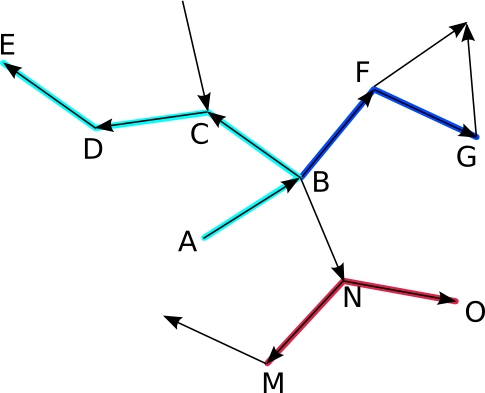
\includegraphics{oriented_graph.png}
 % oriented_graph.png: 485x393 pixel, 300dpi, 4.11x3.33 cm, bb=0 0 116 94
 \caption{An oriented graph (not a tree!), with edge orientation shown as arrows. Two paths are highlighted (cyan and blue). The cyan path starts at node A and ends at node E. Nodes B, C, D, and E are reachable from A. Node C is the direct successor of B in the cyan path; in the blue path the direct successor of B is F. The segment highlighted in red is \emph{not} a path.}
 \label{fig_oriented_graph}
\end{figure}



In the following, $T$ will be a rooted tree. We'll recall that a tree (rooted or not) is a connected, acyclic graph. By choosing one node to be the root (which we'll note $R$), and orienting all edges away from the root, we get an oriented graph. A \textit{path} along such a graph is a sequence of nodes such that there is an edge between two successive nodes, and that these nodes are ordered in the sequence as they are in the edge. The first node in the path is called the \textit{start} of the path, and the last node is its \textit{end}. We speak of a path \textit{from} the start \textit{to} the end, equivalently we say that the end is \textit{reachable} from the start. The nodes in a path are ordered: if $a$ and $b$ are in a path, then either $a$ is reachable from $b$, or $b$ is reachable from $a$, or $a = b$; furthermore if $a$ is reachable from $b$, then $b$ is \textit{not} reachable from $a$. If an edge connects $a$ to $b$, then $b$ is the \textit{direct successor} of $a$, and $a$ is the \textit{direct predecessor} of $b$
See figure {\ref{fig_oriented_graph}.

Although paths are not sets, we will (somewhat abusively, perhaps) use set notation with paths, unless there is a risk of confusion. Thus is $P$ is a path and $n$ is a node, then $n \in P$ means that $n$ is ``in'' $P$  or ``belongs to'' $P$ (strictly speaking, $n$ is reachable from the start of $P$, and the end of $P$ is reachable from $n$).

Now a few definitions - these are mostly renamings of graph-theoretical concepts, to make them more intuitive for phylogenetic trees. 

\begin{dfn}
\label{def_ancestor}
Let $a$ and $b$ be two different nodes of $T$. We say that $a$ is an \textit{ancestor} of $b$, or (equivalently) that $b$ is a \textit{descendant} of $a$, if and only if there is a path from $a$ to $b$. 
\end{dfn}

\begin{dfn}
\label{def_parent}
Let $P$ be a path in $T$, and $a, b$ two nodes in $P$ such that $b$ is the direct successor of $a$. We will call $a$ the \textit{parent} of $b$. We can say \textit{the} parent (rather than \textit{a} parent) of $b$ because i) $a$ lies on the path from $R$ to $b$ (which is unique), and ii) only one node on any path can be another node's direct predecessor. We also see that any node's parent is also its ancestor (which shouldn't be too surprising\ldots), since $b$ is reachable from $a$
\end{dfn}

\begin{dfn}
\label{def_child}
Let $P$ be a path in $T$, and $a, b$ two nodes in $P$ such that $b$ is the direct successor of $a$. We say that $b$ is a \textit{child} of $a$.
\end{dfn}

Note that a node has exactly one parent, except the root which has none. A node can have zero or more children, but we rarely ever encounter nodes with a single child. A node with no children is called a \textit{leaf}.

\begin{dfn}
\label{def_lineage}
A path that starts from the root we call a \emph{lineage}. By the definition of a rooted tree, there is always a lineage to $n$ for any node $n$, and this lineage is unique. So we can unambiguously talk of \textit{the} lineage of $n$ to mean the path from $R$ to $n$. We say that a set $L$ of nodes form a lineage if there exists $n \in L$ such that the path from $R$ to $n$ contains all and only elements of $L$.
\end{dfn}

\begin{figure}[b]
 \centering
 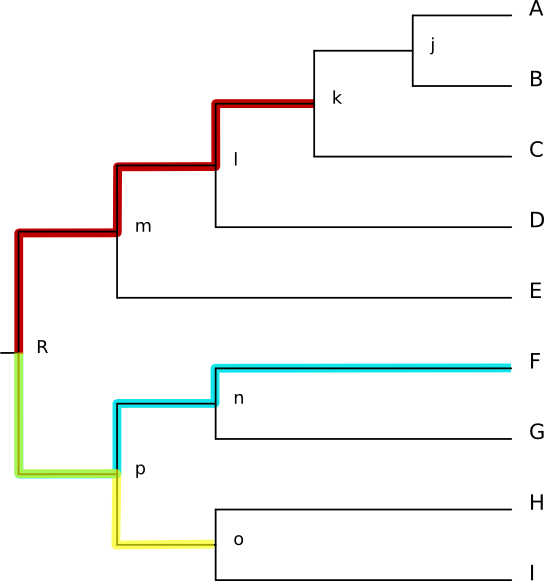
\includegraphics{prop_tree.png}
  \caption{A rooted tree}
 \label{fig_app_tree_prop}
\end{figure}

\begin{prop}
\label{prop_lineage_ancestors_equivalence}
Let $n$ be a node of $T$, and $L$ its lineage. Then all ancestors of $n$ belong to $L$, and all nodes of $L$, except $n$ itself, are ancestors of $n$.
\end{prop}

\begin{proof}

$\Rightarrow$ Let $a$ be an ancestor of $n$. By definition \ref{def_ancestor}, there is a path from $a$ to $n$. By tree properties, there is a path from $R$ to $a$. Hence $a$ belongs to the path from $R$ to $n$, which is the lineage of $n$.
\end{proof}

\noindent{}$\Leftarrow$ Let $l \neq n$ be a node in $L$. Since $L$ is the path from $R$ to $n$, $n$ is reachable from $a$, and hence $a$ is an ancestor of $n$ by definition \ref{def_ancestor}.

\begin{dfn}
If $L$ and $M$ are lineages of $T$, then the \textit{intersection}
of $L$ and $M$, noted $L \cap M$, is the set of nodes that belong to both $L$ and $M$.
\end{dfn} 

\begin{lemma}
\label{lem_ancestors_in_lineage}
Let $n$ be a node of $T$, $L$ its lineage, and $l$ a node of $L$. Then $l$'s ancestors also belong to $L$.
\end{lemma}
\begin{proof}
If $l = n$ then the ancestors of $l$ are those of $n$, which belong to $L$ by proposition \ref{prop_lineage_ancestors_equivalence}. If $l \neq n$ then let $a$ be an ancestor of $l$. By definition \ref{def_ancestor}, $l$ is reachable from $a$. By proposition \ref{prop_lineage_ancestors_equivalence}, $l$ is an ancestor of $n$ and again $n$ is reachable from $l$. Therefore, $n$ is reachable from $a$, so $a$ is an ancestor of $n$, and so belongs in $L$.
\end{proof}

\begin{lemma}
Let $L$ and $M$ be lineages of $T$, and $q \in L \cap M, q \neq R$. Then $q$'s parent also belongs to $M \cap L$.
\end{lemma}
\begin{proof}
Call $p$ the parent of $q$. $p$ is an ancestor of $q$, and since $q$ belongs to $L$ (by hypothesis), $p$ belongs to $L$ by lemma \ref{lem_ancestors_in_lineage}. By the same reasoning, $p$ belongs to $M$, therefore $p \in L \cap M$.

\end{proof}


\begin{prop}
\label{prop_lineage_intersection}
Let $L$ and $M$ be lineages of $T$. Then $L \cap M$ also forms a lineage.
\end{prop}
\begin{proof}
Let $N = L \cap M$. Because $N$ is a subset of a lineage (in fact it is a subset of at least two lineages, $L$ and $M$), its elements are ordered, so we can pick the last one and call it $n$. Now all other elements of $N$ are ancestors of $n$, so by lemma \ref{lem_ancestors_in_lineage} they belong in $L$ and in $M$. So far we have proven 
\end{proof}

\begin{prop}
In a rooted tree, you can always define a clade by specifying a single node: the clade consists of the specified node and all its descendants.
\end{prop}

\begin{prop}
In a rooted tree $T$ with unique labels and a node $n$ in $T$, it is always possible to choose two nodes $n_1$ and $n_2$ such that lca($n_1$,$n_2$) = $n$.
\end{prop}

\end{document}
